\subsection{Arsitektur yang Mengoptimalkan PostgreSQL (PGP)}

\begin{figure}[htbp]
    \centering
    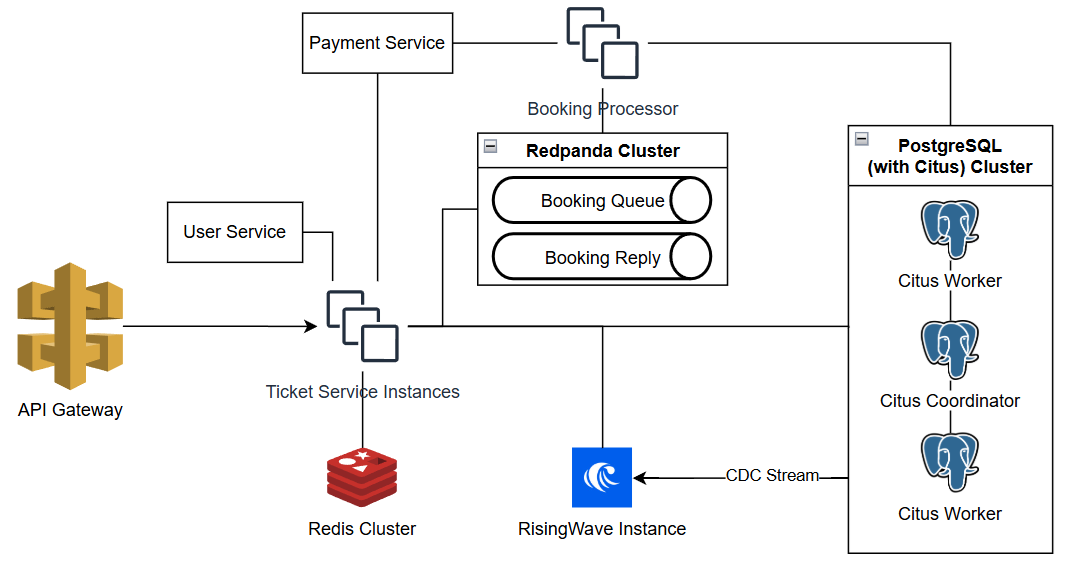
\includegraphics[width=0.8\textwidth]{resources/appendix/architecture-optimized.png}
    \caption{Arsitektur yang Mengoptimalkan PostgreSQL}
    \label{fig:optimized-architecture}
\end{figure}

Arsitektur ini mengoptimalkan sistem dengan pola CQRS. Tanggung jawab permintaan baca dilimpahkan kepada RisingWave. \textit{Streaming database} ini mengonsumsi \textit{CDC stream} dari kluster PostgreSQL, lalu memperbarui kueri secara inkremental. Hal yang perlu diperhatikan dalam penggunaan RisingWave adalah \textit{replication lag}. Data yang dikembalikan oleh RisingWave tidak valid apabila data tersebut \textit{outdated}. Penggunaan ekstensi Citus memungkinkan pembagian data berdasarkan baris dan \textit{multiple writer}. Selain itu, perintah pemesanan tiket (berupa \textit{command}/ \textit{event sourcing}) akan dimasukkan ke dalam antrean terlebih dahulu, lalu diproses secara bertahap. Redis digunakan untuk menyimpan \textit{uncommited data} dan menolak permintaan pemesanan lebih awal.

Penggunaan ekstensi Citus memungkinkan peningkatan \textit{write throughput} tidak hanya dengan pendekatan \textit{scale up}, tetapi juga dengan pendekatan \textit{scale-out}. Redpanda dapat dibuat kluster dengan pemartisian data untuk meningkatkan \textit{throughput}.

\textit{Persistence} pada Redis bersifat asinkron, sehingga terdapat kemungkinan data hilang ketika terjadi kegagalan. Meskipun begitu, penggunaan \textit{key-value store} lain yang \textit{persistent} berpotensi memperlambat kinerja. Dalam kasus ini, Redis akan dikonfigurasikan dalam mode kluster untuk redundansi dan mode AOF untuk \textit{persistence}. Hilangnya data hanya akan terjadi ketika \textit{master} dan \textit{replica} mengalami kegagalan dalam satu waktu. Selain itu, hilangnya data pada Redis tidak akan mengganggu integritas data karena pemeriksaan kedua masih akan dilakukan saat pemrosesan data.

Terdapat isu \textit{fairness} yang harus diperhatikan ketika menggunakan Redpanda sebagai \textit{queue}. Redpanda hanya menjamin \textit{ordering} dalam satu partisi yang sama dan tidak menjamin \textit{ordering} secara global dalam satu topik. Oleh karena itu, pemartisian harus dikonfigurasikan berdasarkan kategori tiket. Dengan pendekatan ini, urutan pemrosesan pada \textit{queue} akan sesuai dengan urutan \textit{request}.